% Options for packages loaded elsewhere
% Options for packages loaded elsewhere
\PassOptionsToPackage{unicode}{hyperref}
\PassOptionsToPackage{hyphens}{url}
\PassOptionsToPackage{dvipsnames,svgnames,x11names}{xcolor}
%
\documentclass[
  letterpaper,
  DIV=11,
  numbers=noendperiod]{scrartcl}
\usepackage{xcolor}
\usepackage{amsmath,amssymb}
\setcounter{secnumdepth}{-\maxdimen} % remove section numbering
\usepackage{iftex}
\ifPDFTeX
  \usepackage[T1]{fontenc}
  \usepackage[utf8]{inputenc}
  \usepackage{textcomp} % provide euro and other symbols
\else % if luatex or xetex
  \usepackage{unicode-math} % this also loads fontspec
  \defaultfontfeatures{Scale=MatchLowercase}
  \defaultfontfeatures[\rmfamily]{Ligatures=TeX,Scale=1}
\fi
\usepackage{lmodern}
\ifPDFTeX\else
  % xetex/luatex font selection
\fi
% Use upquote if available, for straight quotes in verbatim environments
\IfFileExists{upquote.sty}{\usepackage{upquote}}{}
\IfFileExists{microtype.sty}{% use microtype if available
  \usepackage[]{microtype}
  \UseMicrotypeSet[protrusion]{basicmath} % disable protrusion for tt fonts
}{}
\makeatletter
\@ifundefined{KOMAClassName}{% if non-KOMA class
  \IfFileExists{parskip.sty}{%
    \usepackage{parskip}
  }{% else
    \setlength{\parindent}{0pt}
    \setlength{\parskip}{6pt plus 2pt minus 1pt}}
}{% if KOMA class
  \KOMAoptions{parskip=half}}
\makeatother
% Make \paragraph and \subparagraph free-standing
\makeatletter
\ifx\paragraph\undefined\else
  \let\oldparagraph\paragraph
  \renewcommand{\paragraph}{
    \@ifstar
      \xxxParagraphStar
      \xxxParagraphNoStar
  }
  \newcommand{\xxxParagraphStar}[1]{\oldparagraph*{#1}\mbox{}}
  \newcommand{\xxxParagraphNoStar}[1]{\oldparagraph{#1}\mbox{}}
\fi
\ifx\subparagraph\undefined\else
  \let\oldsubparagraph\subparagraph
  \renewcommand{\subparagraph}{
    \@ifstar
      \xxxSubParagraphStar
      \xxxSubParagraphNoStar
  }
  \newcommand{\xxxSubParagraphStar}[1]{\oldsubparagraph*{#1}\mbox{}}
  \newcommand{\xxxSubParagraphNoStar}[1]{\oldsubparagraph{#1}\mbox{}}
\fi
\makeatother


\usepackage{longtable,booktabs,array}
\newcounter{none} % for unnumbered tables
\usepackage{calc} % for calculating minipage widths
% Correct order of tables after \paragraph or \subparagraph
\usepackage{etoolbox}
\makeatletter
\patchcmd\longtable{\par}{\if@noskipsec\mbox{}\fi\par}{}{}
\makeatother
% Allow footnotes in longtable head/foot
\IfFileExists{footnotehyper.sty}{\usepackage{footnotehyper}}{\usepackage{footnote}}
\makesavenoteenv{longtable}
\usepackage{graphicx}
\makeatletter
\newsavebox\pandoc@box
\newcommand*\pandocbounded[1]{% scales image to fit in text height/width
  \sbox\pandoc@box{#1}%
  \Gscale@div\@tempa{\textheight}{\dimexpr\ht\pandoc@box+\dp\pandoc@box\relax}%
  \Gscale@div\@tempb{\linewidth}{\wd\pandoc@box}%
  \ifdim\@tempb\p@<\@tempa\p@\let\@tempa\@tempb\fi% select the smaller of both
  \ifdim\@tempa\p@<\p@\scalebox{\@tempa}{\usebox\pandoc@box}%
  \else\usebox{\pandoc@box}%
  \fi%
}
% Set default figure placement to htbp
\def\fps@figure{htbp}
\makeatother





\setlength{\emergencystretch}{3em} % prevent overfull lines

\providecommand{\tightlist}{%
  \setlength{\itemsep}{0pt}\setlength{\parskip}{0pt}}



 


\usepackage{fancyhdr}
\pagestyle{fancy}
\fancyhf{}
\lhead{STAT 218}
\chead{Chapter 2}
\rhead{Fall 2026}
\rfoot{\thepage}
\setlength{\headheight}{14pt}
\KOMAoption{captions}{tableheading}
\makeatletter
\@ifpackageloaded{caption}{}{\usepackage{caption}}
\AtBeginDocument{%
\ifdefined\contentsname
  \renewcommand*\contentsname{Table of contents}
\else
  \newcommand\contentsname{Table of contents}
\fi
\ifdefined\listfigurename
  \renewcommand*\listfigurename{List of Figures}
\else
  \newcommand\listfigurename{List of Figures}
\fi
\ifdefined\listtablename
  \renewcommand*\listtablename{List of Tables}
\else
  \newcommand\listtablename{List of Tables}
\fi
\ifdefined\figurename
  \renewcommand*\figurename{Figure}
\else
  \newcommand\figurename{Figure}
\fi
\ifdefined\tablename
  \renewcommand*\tablename{Table}
\else
  \newcommand\tablename{Table}
\fi
}
\@ifpackageloaded{float}{}{\usepackage{float}}
\floatstyle{ruled}
\@ifundefined{c@chapter}{\newfloat{codelisting}{h}{lop}}{\newfloat{codelisting}{h}{lop}[chapter]}
\floatname{codelisting}{Listing}
\newcommand*\listoflistings{\listof{codelisting}{List of Listings}}
\makeatother
\makeatletter
\makeatother
\makeatletter
\@ifpackageloaded{caption}{}{\usepackage{caption}}
\@ifpackageloaded{subcaption}{}{\usepackage{subcaption}}
\makeatother
\usepackage{bookmark}
\IfFileExists{xurl.sty}{\usepackage{xurl}}{} % add URL line breaks if available
\urlstyle{same}
% fallback for those not using the hyperref driver hyperxmp:
\makeatletter
\@ifundefined{xmpquote}{\newcommand{\xmpquote}[1]{#1}}{}
\makeatother
\hypersetup{
  colorlinks=true,
  linkcolor={blue},
  filecolor={Maroon},
  citecolor={Blue},
  urlcolor={Blue},
  pdfcreator={LaTeX via pandoc}}


\author{}
\date{}
\begin{document}


\section{Sampling from a Finite
Population}\label{sampling-from-a-finite-population}

\subsection{Definitions}\label{definitions}

\textbf{Population}

\begin{itemize}
\item
  Entire collection of observational units we are interested in
\item
  Relates to the \_\_\_\_\_\_\_\_\_\_\_
\end{itemize}

\textbf{Sample}

\begin{itemize}
\item
  A subset of the population
\item
  Relates to the \_\_\_\_\_\_\_\_\_\_\_
\end{itemize}

\textbf{Generalizations}

\begin{itemize}
\tightlist
\item
  Not only to describe a sample, but to generalize characteristics of a
  sample to a much larger population
\end{itemize}

\subsection{Sampling}\label{sampling}

A sample is considered to be a \_\_\_\_\_\_\_\_\_\_\_\_\_\_\_ sample if
it is like or represents the whole population from which it has been
drawn.

\begin{itemize}
\tightlist
\item
  Would our class be representative of all UNL students?
\end{itemize}

Bias is when a statistic \_\_\_\_\_\_\_\_\_\_\_\_\_\_ overestimates or
underestimates the population for the parameter of interest.

\begin{itemize}
\tightlist
\item
  Would asking UNL students enrolled in 8 am classes if they are morning
  people be representative of all UNL students?
\end{itemize}

\subsection{Sampling Methods}\label{sampling-methods}

\begin{enumerate}
\def\labelenumi{\arabic{enumi}.}
\item
  \textbf{Convenience Sampling}

  \begin{itemize}
  \item
    Go and pick out a set of observational units
  \item
    Not a very good way to select a sample because this will introduce
    \_\_\_\_\_\_\_
  \item
    Example: taking surveys outside of the cafeteria
  \end{itemize}
\item
  \textbf{Simple Random Sample}

  \begin{itemize}
  \item
    Every population member has an equal probability of being chosen
  \item
    Allows us to \_\_\_\_\_\_\_\_\_\_\_\_\_\_\_\_ our results to the
    entire population
  \item
    Choose individuals randomly from the sampling frame and each
    individual has the same chance of being selected
  \item
    \textbf{Sampling frame:} \_\_\_\_\_\_ of all individuals in the
    population of interest
  \end{itemize}
\end{enumerate}

\textbf{Example 1:} Researchers at UNL are looking for student feedback
(approval/disapproval) regarding an upcoming project. They set up a
table outside of each dorm hall and ask passing students for their
input. The volunteers at the table talk to any student who is interested
in providing feedback.

\begin{itemize}
\item
  Identify the following

  \begin{itemize}
  \item
    Population:
  \item
    Parameter of interest:
  \item
    Sampling Frame:
  \item
    Sample:
  \item
    Potential Bias:
  \end{itemize}
\end{itemize}

\textbf{Example 2:} A business magazine mailed a questionnaire to the
human resources of all the Fortune 500 companies and received responses
from 23\% of them. Those responding reported that they did not find that
such surveys intruded significantly on their workday.

\begin{itemize}
\item
  Identify the following

  \begin{itemize}
  \item
    Population:
  \item
    Parameter of interest:
  \item
    Sampling Frame:
  \item
    Sample:
  \item
    Potential Bias:
  \end{itemize}
\end{itemize}

\textbf{Example 3:} State police set up a roadblock to check cars for
up-to-date registration and insurance. They usually find problems in
about 10\% of the cars they stop.

\begin{itemize}
\item
  Identify the following:

  \begin{itemize}
  \item
    Population:
  \item
    Parameter of interest
  \item
    Sampling Frame:
  \item
    Sample:
  \item
    Potential Bias:
  \end{itemize}
\end{itemize}

\section{Inference for a Single Quantitative
Variable}\label{inference-for-a-single-quantitative-variable}

\subsection{Definitions}\label{definitions-1}

Summary Statistics: statistics calculated from a sample that provide
numeric information about the sample

\begin{itemize}
\item
  Mean / Average

  \begin{itemize}
  \tightlist
  \item
    Add up all the values first, then divide by the total number of
    values
  \end{itemize}
\item
  Median

  \begin{itemize}
  \item
    Half of the data is above, half is below
  \item
    ``Middle'' value when data is ordered
  \end{itemize}
\item
  Outliers: unusual data points
\end{itemize}

A summary statistic is called \_\_\_\_\_\_\_\_\_\_\_\_\_\_ if its value
does not change much when outliers are included

Example: Suppose that the following values are observed. Calculate the
mean and median.

\[
8,10,11,12,15,7,8,9
\]

\hfill\break
\hfill\break
\hfill\break
\hfill\break
\hfill\break

Suppose that instead of 15, the value 30 was observed. Calculate the
mean and the median.

\hfill\break
\hfill\break
\hfill\break
\hfill\break
\hfill\break

Note: The standard deviation will \_\_\_\_\_\_\_\_\_\_\_\_\_ if an
outlier is added to the data set.

\subsection{Symbols}\label{symbols}

{\def\LTcaptype{none} % do not increment counter
\begin{longtable}[]{@{}
  >{\raggedright\arraybackslash}p{(\linewidth - 4\tabcolsep) * \real{0.1806}}
  >{\centering\arraybackslash}p{(\linewidth - 4\tabcolsep) * \real{0.2639}}
  >{\centering\arraybackslash}p{(\linewidth - 4\tabcolsep) * \real{0.2639}}@{}}
\toprule\noalign{}
\begin{minipage}[b]{\linewidth}\raggedright
\end{minipage} & \begin{minipage}[b]{\linewidth}\centering
\textbf{Quantitative}
\end{minipage} & \begin{minipage}[b]{\linewidth}\centering
\textbf{Categorical}
\end{minipage} \\
\midrule\noalign{}
\endhead
\bottomrule\noalign{}
\endlastfoot
Population & \(\mu\) & \(\pi\) \\
Sample & \(\overline{x}\) & \(\widehat{p}\) \\
\end{longtable}
}

\subsection{Analysis of a Single Quantitative
Variable}\label{analysis-of-a-single-quantitative-variable}

\textbf{Variable of Interest:}

\begin{itemize}
\tightlist
\item
  Number of \ldots{} context, quantitative
\end{itemize}

\textbf{Parameter:}

\begin{itemize}
\tightlist
\item
  ``The long run \textbf{average}\ldots{}\emph{context''} (\(\mu\))
\end{itemize}

\textbf{Hypotheses:}

\begin{itemize}
\item
  Words:

  \begin{itemize}
  \item
    Null: The long-run average \ldots{}\emph{context\ldots{}} is equal
    to previously known \#.
  \item
    Alternative: The long-run average \ldots{}\emph{context\ldots{}} is
    greater than/ less than/ different from previously known \#..
  \end{itemize}
\item
  Symbols:

  \begin{itemize}
  \item
    \(H_{0}:\mu = previously\ known\ \#\)
  \item
    \(H_{A}:\mu > , < , \neq previously\ known\ \#\)
  \end{itemize}
\end{itemize}

\textbf{Example:} Suppose you are interested in whether the average
number of bikes sold at a store per day is less than 20

\begin{itemize}
\item
  \textbf{Variable of interest:} number of bikes sold in a day,
  quantitative
\item
  \textbf{Parameter:} the long-run average number of bikes sold at the
  store (µ)
\item
  \textbf{Hypotheses}

  \begin{itemize}
  \item
    Words

    \begin{itemize}
    \item
      Null: The long-run average number of bikes sold at the store is
      equal to 20
    \item
      Alternative: The long run average number of bikes sold at the
      store is less than 20
    \end{itemize}
  \item
    Symbols

    \begin{itemize}
    \item
      \(H_{0}:\)
    \item
      \(H_{A}:\)
    \end{itemize}
  \end{itemize}
\end{itemize}

For the purposes of our class, we will not use the simulation approach
for quantitative data because we do not have coin flips or spinners to
model quantitative data. This means that we will not calculate p-values.

\subsection{Theory Based Approach
(Quantitative)}\label{theory-based-approach-quantitative}

We need to satisfy at least one of the following conditions to use the
theory approach.

\begin{itemize}
\item
  The quantitative variable should have a symmetric distribution
\item
  Sample size \(\geq\) \_\_\_\_\_ and sampling distribution is not
  strongly skewed
\end{itemize}

Standard Error = \(\frac{s}{\sqrt{n}}\) where s is our sample standard
deviation

Standardized Statistic =
\(\frac{\overline{x} - \mu}{SE} = \frac{\overline{x} - \mu}{\frac{s}{\sqrt{n}}}\)

\subsection{Standardized Statistic for Quantitative
Data}\label{standardized-statistic-for-quantitative-data}

Remember that the standardized statistic calculates how many standard
deviation from the null value that the statistics falls

\begin{itemize}
\tightlist
\item
  For quantitative variables:
\end{itemize}

\[z = \ Standardized\ statistic\  = \frac{sample\ mean\  - null\ value}{standard\ deviation\ of\ sample\ mean} = \ \frac{\overline{x} - \mu_{0}}{\frac{\sigma}{\sqrt{n}}}\]

Since \(\sigma\) is not usually known, we use the sample standard
deviation (s) to approximate the standard deviation of sample mean

\begin{itemize}
\item
  This approximation is called the \textbf{standard error} (SE) of
  sample mean
\item
  t = standardized statistic =
  \(\frac{\overline{x} - \mu}{\frac{s}{\sqrt{n}}}\)
\end{itemize}

Like with the normal approximation, we need a reference distribution.
With categorical data, we used the z (standard normal) distribution.
Since we are now using the sample standard deviation, we need to use the
t distribution instead of the z distribution

One Quantitative Variable

\[SE = \frac{s}{\sqrt{n}} \leftarrow this\ is\ our\ new\ denominator\ for\ standardized\ statistic\]

\[Standardized\ Statistic = t = \frac{\overline{x} - \mu}{\frac{s}{\sqrt{n}}}\]

Note that the cutoffs are the same as Chapter 1: ``outside the 2's
-\textgreater{} reject''

\pandocbounded{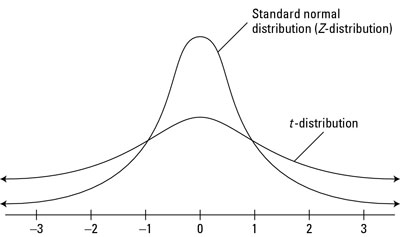
\includegraphics[keepaspectratio]{../images/Notes218_Chapter_2_image3.jpeg}}

\textbf{Example:} You observe the bike sales for 30 days to find the
average number of sales to be 19.5, with a sample standard deviation of
2.1

\(H_{0}:\mu = 20\)

\(H_{A}:\mu < 20\)

Conclusion: ``We \_\_\_\_\_\_ have evidence to conclude the long run
average number of bikes sold at the store is
\_\_\_\_\_\_\_\_\_\_\_\_\_\_\_\_\_\_

\section{Errors and Significance}\label{errors-and-significance}

With all our hypotheses, we made assumptions about the null hypothesis.
Our statistic provided strength of evidence.

Strength of evidence

\begin{itemize}
\item
  Calculate p-value -- Probability of our observed statistic happening
  given the null is true.
\item
  p-value \(< \ 0.05\  \rightarrow\) Reject the Null (suggests the
  alternative)
\item
  p-value \(\geq \ 0.05\  \rightarrow\) Fail to Reject the Null
\end{itemize}

However, some of the null distribution was true even when we rejected
the null hypothesis. How do we classify the instances when we are wrong?
Recall the Buzz and Doris example.

Hypotheses:

\begin{itemize}
\item
  \(H_{O}:\) Buzz is just guessing.
\item
  \(H_{A}:\) Buzz is not guessing (i.e.~they are communicating).
\end{itemize}

\textbf{Type I Error}

\begin{itemize}
\item
  \_\_\_\_\_\_\_\_ the null hypothesis, but in reality the null is
  actually \_\_\_\_\_\_\_\_\_
\item
  False alarm -- believe we have discovered a difference when no
  difference exists
\item
  What would a Type I Error look like for the Buzz and Doris scenario?

  \begin{itemize}
  \tightlist
  \item
    We conclude that Buzz is \emph{not} guessing, but he actually is
    guessing
  \end{itemize}
\end{itemize}

\textbf{Type II Error}

\begin{itemize}
\item
  \_\_\_\_\_\_\_\_\_\_\_\_\_\_\_\_\_ the null, but in reality the null
  is actually \_\_\_\_\_\_\_\_\_\_
\item
  Missed opportunity -- failing to detect difference that is there
\item
  What would a Type II Error look like for the Buzz and Doris scenario?

  \begin{itemize}
  \tightlist
  \item
    We conclude that Buzz is guessing, when Buzz is actually \emph{not}
    guessing
  \end{itemize}
\end{itemize}

In reality, we never know if we made an error or not. However, we can
control what we want to happen: significance level and power.

\subsection{Significance Level (α)}\label{significance-level-ux3b1}

\(\alpha\) (alpha) is our ``threshold'' for p-value (\emph{we have been
using 0.05}).

\begin{itemize}
\item
  How small a p-value needs to be to provide convincing evidence to
  reject the null hypothesis
\item
  p-value \(< \alpha\  \rightarrow\) Reject \(H_{O}\)
\item
  p-value \(\geq \alpha\  \rightarrow\) Fail to Reject \(H_{O}\)
\end{itemize}

Example:

\begin{itemize}
\item
  If \(\alpha = 0.05\), then for a p-value of 0.07, we will fail to
  reject our null.
\item
  If \(\alpha = 0.10\), then for a p-value of 0.07, we will reject our
  null.
\end{itemize}

This value changes depending on the study, your discipline, etc.
Consider a significance level of 0.1. This means, that if the null is
really true, 10\% of random samples would produce a sample statistic
that is extreme enough to reject the null hypothesis.

\(\alpha =\) Probability of Type I Error

\begin{itemize}
\item
  The \_\_\_\_\_\_\_\_\_\_ it is, \_\_\_\_\_\_\_\_\_ likely to make a
  Type I Error
\item
  As the probability of a Type I Error goes \_\_\_\_, the probability of
  a Type II Error goes \_\_\_
\end{itemize}

\subsection{Power}\label{power}

Power is defined as the probability of rejecting a \_\_\_\_\_ null
hypothesis. The calculation of power goes beyond the scope of our class,
but we want power to be as high as possible.

\[Power = 1 - P(Type\ II\ Error)\]

\pandocbounded{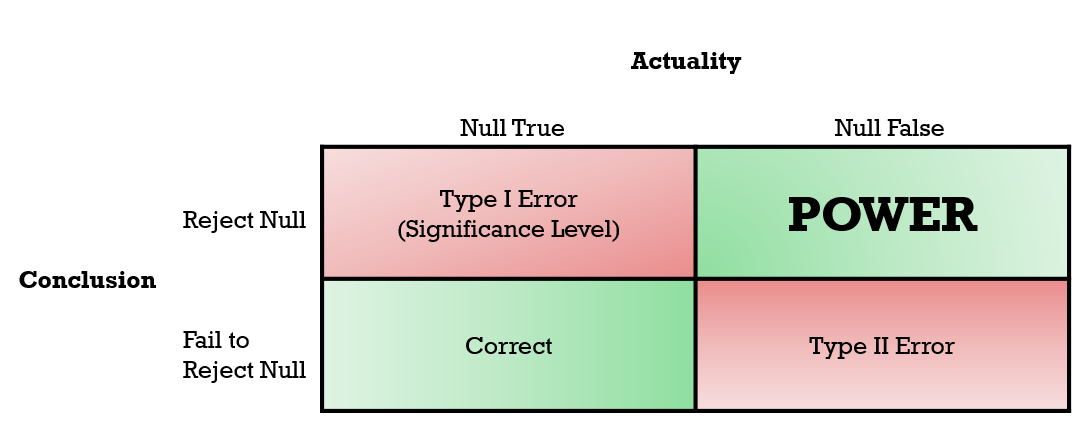
\includegraphics[keepaspectratio]{../images/Notes218_Chapter_2_image6.png}}

Example: Suppose you are implementing an algorithm that detects fraud on
credit cards. From the gathered information, you decide to test the
following hypothesis:

\begin{itemize}
\item
  \(H_{0}:\) No fraud detected
\item
  \(H_{A}:\) Fraud detected
\end{itemize}

In context, describe the impacts of each type of conclusion.

\begin{itemize}
\item
  Reject the null when the null is true (what type of error is this?)
\item
  Reject the null when the null is false
\item
  Fail to reject the null when the null is true
\item
  Fail to reject the null when the null is false.
\end{itemize}




\end{document}
